\chapter{Statistics: Learning to Estimate}
\label{ch:05-statistics-estimation}

\lecturemeta{Kyunghyun Cho}{New York University}

Cho's lecture has one thesis, stated plainly two-thirds of the way through and worth quoting
because it reorganises a great deal of statistics: inference does not have to be about
inverting the generative process. The conventional route to any estimand is to model the data
generating distribution and then invert it, and the lecture's claim is that this step is
optional. Given the ability to sample problems with known answers, estimator design becomes a
supervised regression problem, and gradient descent finds an estimator that beats the textbook
one. The argument is built on a deliberately trivial example, the population standard
deviation, then repeated for mutual information, Bayesian predictive distributions and causal
effects, and finally turned back on theory to redefine what identifiability means.

\section*{Key ideas}

\paragraph{Start with something embarrassingly simple.} The sample standard deviation is a
biased estimate of the population standard deviation, because the square root sits outside
the expectation. Rather than deriving a correction, Cho asks why estimator design is not
simply a minimisation problem. Given pairs $(\mathcal{D}, \params)$ of a sample set and the
true population standard deviation, a good estimator $F$ has low
$\MSE$, and the only source of variation is the sampling that produced $\mathcal{D}$. So
define a meta-distribution $P_\Gamma$ over distributions of known population standard
deviation and minimise over a hypothesis class $\mathcal{F}$ of estimators,
\[
  \min_{F \in \mathcal{F}} \;
  \Ex_{\pi \dist P_\Gamma}\Bigl[\,
    \Ex_{\mathcal{D} \dist \pi}\bigl[\,
      \MSE\bigl( F(\mathcal{D}),\, \mathrm{stdev}(\pi) \bigr)
    \bigr]
  \Bigr].
\]
\noindent As the slides note, this is exactly training a regression model: a data distribution
$P_\Gamma$, a set of samples as input, a real number as output, and an MSE loss.

\paragraph{The architecture is forced by an invariance.} An estimator over a sample set must
be permutation invariant, so $F$ is a transformer with the positional embeddings removed,
followed by aggregation, which the lecture calls Set
Transformer++~\citep{zhang2022setnorm}.\footnote{``Set Transformer++'' is the lecture's own name
for the architecture. The cited paper is on set norm and equivariant skip connections for deep
sets, and does not use that name.} This is a small but neat
instance of the geometric deep learning argument
(Chapter~\ref{ch:11-geometric-deep-learning}): the symmetry of the data dictates the
architecture, here without either speaker mentioning the other.

\paragraph{It works, and the reason it works is the interesting part.} The learned estimator
is essentially unbiased where \texttt{np.std} is not, is more sample-efficient, converges as
the sample size grows, and, importantly, works on log-normal distributions that were held out
of training (Figure~\ref{fig:statistics-estimation-1}). Cho's reading of that last fact is
the pivot of the lecture. Had the network been implicitly identifying the underlying
distribution, fitting it, and then correcting the sample standard deviation, it would fail on
a family it had never seen. It does not fail, so it is doing something else: bypassing
density estimation and going straight to inference. Supervised learning found a new estimator
of the population standard deviation.

\begin{figure}[htbp]
\centering
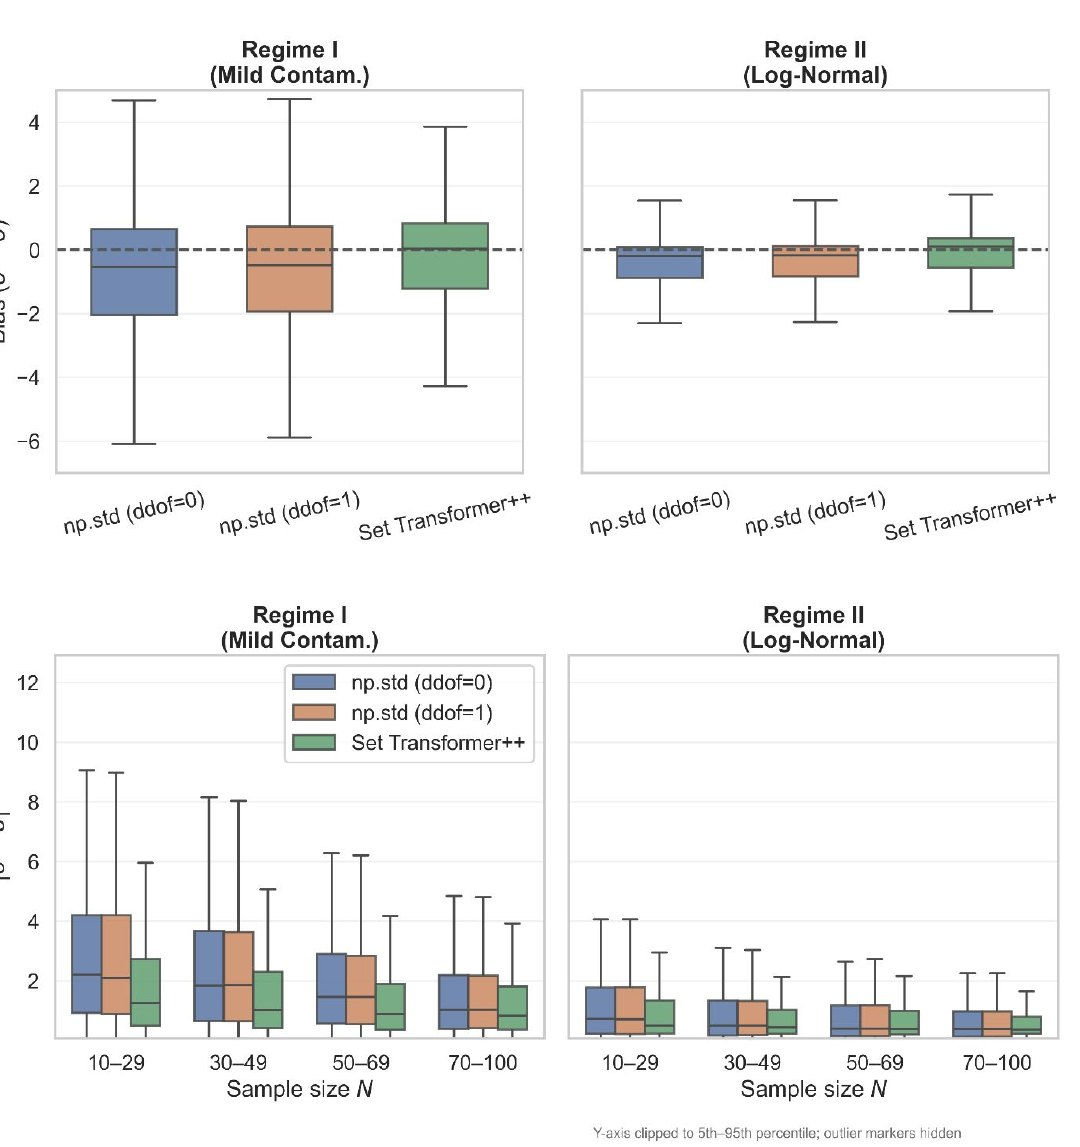
\includegraphics[width=0.60\textwidth]{figures/statistics-estimation-1.jpg}
\caption{The proof of concept from the Statistics lecture. Top, bias
$\est{\sigma} - \sigma$ for two \texttt{numpy} estimators and the learned one, under mild
contamination and under a log-normal regime that was held out of training. Bottom, absolute
error against sample size. The learned estimator is centred on zero where \texttt{np.std} sits
below it, and it holds up on the unseen family, which is the evidence that it is not
implicitly fitting a density.}
\label{fig:statistics-estimation-1}
\end{figure}

\paragraph{The same move, three more times.} Mutual information is defined through density
ratios, so the reflex is to estimate the ratio; MIST instead attends over both the sample
axis and the dimension axis and predicts MI directly, reportedly outperforming existing
estimators, keeping both bias and variance low, largely escaping the curse of dimensionality,
and generalising to dimensionalities and sample sizes outside its training range. Once available,
a learned estimator can itself serve as an objective function. The Bayesian predictive
distribution is defined through the posterior, so the reflex is to approximate the posterior;
prior-data fitted networks approximate the predictive distribution directly with a
transformer~\citep{muller2022pfn}, matching exact Gaussian-process predictions closely at a
fraction of the cost of MCMC. That raises the obvious objection, where did the prior go, and
the answer is to supply it in context: sample a prior, sample datasets from it, and train
multi-task in-context learning to condition on both. Causal effects get the same treatment
under the name black-box causal inference~\citep{bynum2025bbci}, recovering estimators for observed
confounders and for instrument variables, and tested on the LaLonde job-training
data~\citep{lalonde1986}. A
recurring caveat is that diversity of the training prior, not just its correctness,
determines how far the estimator generalises.

\paragraph{Computational identifiability.} The theoretical payoff is a redefinition.
Mathematical identifiability says that if two observations of infinitely many samples have
matching distributions then the parameters of interest must coincide. Cho proposes
\emph{computational} identifiability instead~\citep{bynum2026identifiability}, defined relative to
three operational constraints: a prior over the problem space, a hypothesis space, and an optimisation
algorithm. The procedure is explicit. Take a causal query; define a prior over structural
causal models combining given and simulated distributions; define a hypothesis space
reachable by the chosen optimiser; search for the best estimator; and if it is accurate for most of
the sampled SCMs, declare the query identifiable. Unlike the mathematical version this is
soft, so one can compute $p(\text{identifiable} \given \varepsilon)$ and plot it as a curve.

\section*{Notation}

$\params$ is the estimand, $\est{\params}$ or $F(\mathcal{D})$ the estimate, $\mathcal{D}$ a
sample set, $\pi$ a single data distribution and $P_\Gamma$ the meta-distribution over such
distributions. The distinction between $\pi$ as a distribution over data here and $\pi$ as a
policy in Chapter~\ref{ch:04-intro-reinforcement-learning} is the speakers' own; both are
standard in their fields and neither is changed.

\section*{Why it matters}

This is the most quietly radical lecture of the week, and it cuts against
Chapter~\ref{ch:02-representational-geometry} in a way worth noticing. Isola measures whether
learned representations agree, using fixed metrics as the yardstick; Cho's programme suggests
the yardstick itself should be learned, which is the same instinct as Isola's own remark that
there is no future for unlearned distance functions. Read together they point at a world where
both the model and the measurement are fitted, and where the burden shifts entirely onto the
prior over problems. The bias-variance material also connects to Alistarh's linearity theorem
(Chapter~\ref{ch:10-efficient-learning}), which is another attempt to predict an error rather
than measure it.

\begin{aside}
The load-bearing assumption is easy to miss because the examples are so clean. Every learned
estimator here is only as good as the meta-distribution $P_\Gamma$ it was trained over, and
for the standard-deviation example we can write that prior down honestly. For causal queries
we cannot, which is precisely why computational identifiability is defined relative to a
prior rather than absolutely. That makes it an honest notion, but it also means a query can
be declared identifiable under one prior and not another, and the lecture does not claim
otherwise.
\end{aside}
